%%%%%%%%%%%%%%%%%%%%%%% file template.tex %%%%%%%%%%%%%%%%%%%%%%%%%
%
% This is a general template file for the LaTeX package SVJour3
% for Springer journals.          Springer Heidelberg 2014/09/25
%
% Copy it to a new file with a new name and use it as the basis
% for your article. Delete % signs as needed.
%
% This template includes a few options for different layouts and
% content for various journals. Please consult a previous issue of
% your journal as needed.
%
%%%%%%%%%%%%%%%%%%%%%%%%%%%%%%%%%%%%%%%%%%%%%%%%%%%%%%%%%%%%%%%%%%%
% First comes an example EPS file -- just ignore it and
% proceed on the \documentclass line
%% your LaTeX will extract the file if required
\begin{filecontents*}{example.eps}
%%!PS-Adobe-3.0 EPSF-3.0
%%%BoundingBox: 19 19 221 221
%%%CreationDate: Mon Sep 29 1997
%%%Creator: programmed by hand (K)
%%%EndComments
%%
gsave
newpath
  20 20 moveto
  20 220 lineto
  220 220 lineto
  220 20 lineto
closepath
2 setlinewidth
gsave
  .4 setgray fill
grestore
stroke
grestore
\end{filecontents*}
%
\RequirePackage{fix-cm}
%
\documentclass{svjour3}                     % onecolumn (standard format)
%\documentclass[smallcondensed]{svjour3}     % onecolumn (ditto)
%\documentclass[smallextended]{svjour3}       % onecolumn (second format)
%\documentclass[twocolumn]{svjour3}          % twocolumn
%\documentclass[referee]{svjour3} 
\smartqed  % flush right qed marks, e.g. at end of proof
%
\usepackage{amsmath}
\usepackage{graphicx}
\usepackage{lineno}
\usepackage{natbib}
\linenumbers
%
% \usepackage{mathptmx}      % use Times fonts if available on your TeX system
%
% insert here the call for the packages your document requires
%\usepackage{epstopdf}
%\graphicspath{ {./images/results} }
\usepackage{color}
%\usepackage{ctable}
%\usepackage{epsfig}
%\usepackage{hyperref}
%\usepackage{soul}
%\usepackage{amssymb}
% etc.
%
% please place your own definitions here and don't use \def but
% \newcommand{}{}
%
% Insert the name of "your journal" with
 \journalname{Boundary-Layer Meteorology Research Note}

%
\newcommand*\patchAmsMathEnvironmentForLineno[1]{%
\expandafter\let\csname old#1\expandafter\endcsname\csname #1\endcsname
\expandafter\let\csname oldend#1\expandafter\endcsname\csname end#1\endcsname
\renewenvironment{#1}%
{\linenomath\csname old#1\endcsname}%
{\csname oldend#1\endcsname\endlinenomath}}% 
\newcommand*\patchBothAmsMathEnvironmentsForLineno[1]{%
\patchAmsMathEnvironmentForLineno{#1}%
\patchAmsMathEnvironmentForLineno{#1*}}%
\AtBeginDocument{%
\patchBothAmsMathEnvironmentsForLineno{equation}%
\patchBothAmsMathEnvironmentsForLineno{align}%
\patchBothAmsMathEnvironmentsForLineno{flalign}%
\patchBothAmsMathEnvironmentsForLineno{alignat}%
\patchBothAmsMathEnvironmentsForLineno{gather}%
\patchBothAmsMathEnvironmentsForLineno{multline}%
}


% ---------------------------------------------------------------------------------------------------------------------------------
% ---------------------------------------------------------------------------------------------------------------------------------
\begin{document}

\title{On the solution of katabatic flows with spatially varying eddy viscosity and diffusivity}

\titlerunning{Exact analytic solution for slope flows}        % if too long for running head


%\authorrunning{Short form of author list} % if too long for running head
\author{M.~G.~Giometto \and R.~Grandi\and J.~Fang \and M.~B.~Parlange}

\institute{ M.~G.~Giometto \at School of Architecture, Civil and Environmental Engineering, \'Ecole Polytechnique F\'ed\'erale de Lausanne, Lausanne, Switzerland \\
		\email{marco.giometto@epfl.ch}
		\and
		R.~Grandi \at Mathematics Institute for Geometry and Applications, \'Ecole Polytechnique F\'ed\'erale de Lausanne, Lausanne, Switzerland \\
		 \and 
		 J.~Fang \at School of Architecture, Civil and Environmental Engineering, \'Ecole Polytechnique F\'ed\'erale de Lausanne, Lausanne, Switzerland \\
		 \and
		M.~B.~Parlange \at Dept. of Civil Engineering, Faculty of Applied Science, University of British Columbia, Vancouver, BC, Canada
}

\date{Received: DD Month YEAR / Accepted: DD Month YEAR}
% The correct dates will be entered by the editor


\maketitle

% ABSTRACT
\begin{abstract}
The Nieuwstadt closed form solution for the stationary Ekman layer is generalized for katabatic flows within the conceptual framework of the Prandtl model. 
The solution is valid for spatially-varying eddy viscosity and diffusivity (O'Brien type) and constant Prandtl number $(Pr)$. 
Momentum and buoyancy transfer coefficients are specified in accordance with Monin-Obukhov similarity.
The characteristics of the solution are discussed as a function of the dimensionless model parameters $Pr$ and $\hat{z}_0 \hat{N}^2 \hat{b}_s^{-1}$, where $\hat{z}_0$ is the hydrodynamic roughness length, $\hat{b}_s$ is the imposed surface buoyancy and $\hat{N}$ is the Brunt-V\"ais\"al\"a frequency.
For the considered range of such parameters, velocity and buoyancy profiles show significant variations in both phase and amplitude of extrema with respect to the classic constant-$K$ model and a more recent approximate solution based on the Wentzel-Kramers-Brillouin (WKB) theory.
Near-wall regions are characterized by relatively stronger surface momentum and buoyancy gradients, whose magnitude is inversely proportional to $Pr$. In addition, slope-parallel momentum and buoyancy fluxes are reduced, the low-level jet (LLJ) is further displaced toward the wall, and its peak velocity strongly depends on $\hat{z}_0 \hat{N}^2 \hat{b}_s^{-1}$.

%Simple approximate functions (based on the new solution) are provided, to relate the internal parameters of the system $(u_*, b_*)$ to the given external parameters.
%Universal functions are also provided to describe the variation of $ z_j$, $z_r$, and $\max{(u)}$, as a function of the dimensionless model parameter $z_0$.
\end{abstract}


\section{Introduction}
Slope winds are ubiquitous in nature and engineering, and they are of interest not only as a fundamental problem in itself, but also because of the important role they play over a broad range of scales and applications. 
On a local scale, for instance, they regulate local weather conditions, influencing atmospheric transport of momentum and scalars such as heat and humidity \citep{whiteman1990, Whiteman, Monti2002, Nylen2004b, Rotach2007, Lehner2015}. 
On a regional scale, they can be responsible for intense cyclonic vorticity in the middle and upper troposphere \citep{Parish1991, Parish1992, Parish1998}.
Persistent katabatic winds characterize the atmospheric boundary layer over Antarctica \citep{Chu1987, Renfrew2004, Renfrew2006a} and over glaciers \citep{Oerlemans1993, Oerlemans1994, pastex1994, Greuell1997, Smeets1997, Oerlemans1998, oerlemans1999, Smeets2000, Oerlemans2002}. Therefore an accurate characterization of such flows is an essential component of understanding and modeling of the weather and climate.
The problematic geometrical setup complicates measurements \citep{Oldroyd2015}, whereas the complex dynamics (e.g. turbulent intermittency, waves, Kelvin-Helmholtz instabilities, low-level jets) and the lack of a satisfactory similarity theory for such flows \citep{Nadeau2012} pose a challenge in terms of computational requirements for numerical modelers. In most cases the required resolution is in fact prohibitively costly \citep{Fedorovich2009, Fedorovich2009d, burkholder_2011}.
Because of this, conceptual models are still of great interest, and represent a valid tool for the characterization of such systems. 

A cornerstone in the understanding of slope flows is represented by the classic Prandtl analytic model \citep{Prandtl}, afterwards extended to include Coriolis force \citep{Gutman1964}, external winds \citep{Lykosov_1972}, and surface variability \citep{Shapiro2007, Oldroyd2014,Zardi2015}, to name but a few.
The Prandtl model approximates the atmosphere in a Boussinesq sense and describes a steady stratified flow over a thermally perturbed unbounded planar sloping surface. It is summarized by the following system of ordinary differential equations:
%
\begin{linenomath*}
\begin{subequations}
	\begin{align}
	- \hat{N}^2 \hat{u}(\hat{z}) \sin{\alpha} & = [ \hat{K}_H \hat{b}_{\hat{z}} ]_{\hat{z}} \, , \\
	\hat{b}(\hat{z}) \sin{\alpha} & = [ \hat{K}_M \hat{u}_{\hat{z}} ]_{\hat{z}} \, ,
	\end{align}
	\label{Prandtl_eq}
\end{subequations}
\end{linenomath*}
%
where $\hat{(\cdot)}$ is used to denote a dimensional variable or parameter, $(\cdot)_{\hat{z}}$ denotes differentiation with respect to the slope-normal coordinate direction $\hat{z}$, $\hat{u}$ is the downslope velocity, $\hat{b} \equiv \hat{g} \hat{\theta}^{\prime} / \hat{\theta}_0$ is buoyancy, where $\hat{g}$ is the gravitational acceleration, $\hat{\theta}^{\prime}$ is the potential temperature perturbation (with respect to the background stably stratified environment characterized by the Brunt-V\"ais\"al\"a frequency $\hat{N}$), and $\hat{\theta}_0$ is a reference (constant) temperature; $\alpha$ is the slope angle and $\hat{K}_M$ and $\hat{K}_H$ denote the eddy viscosity and diffusivity (a model is used to parametrize turbulent fluxes of momentum and buoyancy, respectively).
Equations are defined in $\hat{z} \in \ [\hat{z}_0,\infty)$ with boundary conditions $\hat{u}(\hat{z}_0)=0$, $\hat{u}(\hat{z} \rightarrow \infty) = 0$, $\hat{b}(\hat{z}_0)=\hat{b}_s$ and $\hat{b}(\hat{z} \rightarrow \infty) = 0$ ($\hat{b}_s > 0$ for upslope flows, whereas $\hat{b}_s<0$ for downslope flows). 
Eqs. 1 state that the slope-parallel component of buoyancy is balanced by momentum flux divergence, and that slope-parallel buoyancy advection is balanced by buoyancy flux divergence.
The flow is assumed to be invariant in the along-slope direction and the model can be used to determine the slope-normal $(\hat{z})$ structure of velocity $\hat{u}(\hat{z})$ and buoyancy $\hat{b}(\hat{z})$.
The model is applicable far enough away from ridges and valleys that non-linear advection terms become small \citep{NAPPO1987}, and a balance between advection and diffusion (of both momentum and buoyancy) is achieved. This constraint is rather restrictive, as shown in \citet{Zardi2015}. 
The Prandtl constant-K solution reads 
%
\begin{linenomath*}
\begin{subequations}
	\label{Prandtl_sol}
	\begin{align}
		\hat{b} & = \hat{b}_s \exp{(-\hat{\sigma}_c \hat{z})} \cos{(\hat{\sigma}_c \hat{z})} \, , \\
		\hat{u} & = -\frac{\hat{b}_s}{N Pr} \exp{(-\hat{\sigma}_c \hat{z})} \sin{(\hat{\sigma}_c \hat{z})} \, ,
	\end{align}
\end{subequations}
\end{linenomath*}
%
where
%
\begin{eqnarray}
	\hat{\sigma}_c^2 \equiv \frac{\hat{\sigma_0}}{2\hat{K_H}} \, , \qquad \mathrm{and} \qquad
	\hat{\sigma}_0 \equiv \frac{\hat{N} \sin{(\alpha)}}{\sqrt{Pr}} \, .
\end{eqnarray}
%
The model is able to represent the low-level jet (LLJ) and the return flow region, key features of observed katabatic and anabatic flows. 
However, the constant-K solution is also known to be over-dissipative in the near-surface regions, and under dissipative above the LLJ regions \citep{Defant1949,Oerlemans1998, grisogono2001katabatic}. It is therefore not able to represent the observed strong surface gradients of temperature and momentum, and, in addition, the predicted wind speed typically decreases too rapidly away from the surface.
Simple variations in the eddy diffusivity profiles were introduced in a patched analytic solution by \citet{gutman_1983}, whereas more recently \citet{grisogono2001katabatic} considered general variations in the vertical structure of the eddy diffusivities, and derived  a patched global solution based on the WKB approximation \citep{Bender1979}.
The WKB solution to the Prandtl equations, valid to leading-order in the inner layer and to first-order in the outer layer, reads
%
\begin{subequations}
	\begin{align}
		\hat{f}_{in} & \sim  \exp{ \left( -(1 \pm i) (\hat{\sigma}_0/2)^{1/2} \int_0^{\hat{z}}{\hat{K}_H(z)^{-1/2}}{\mathrm{d}z}\right)}  &  \hat{z} \in [\hat{z}_0,\hat{h}] \, , \\
		\hat{f}_{out}&  \sim  [ \hat{K}_H(\hat{z}) / \hat{K}_H(\hat{h}) ]^{-1/4} \exp{ \left( -(1 \pm i) (\hat{\sigma}_0/2)^{1/2} \int_0^{\hat{z}}{\hat{K}_H(z)^{-1/2}}{\mathrm{d}z} \right)} & \hat{z} \in [\hat{h},\infty) \, ,
	\end{align}
	\label{WKB_sol}
\end{subequations}
%
where $\hat{f}_{in} \equiv \hat{b}_{in}+ i\hat{u}_{in}$ represents the inner-layer solution, and $\hat{f}_{out} \equiv \hat{b}_{out} + i\hat{u}_{out}$ is the outer-layer solution. $\hat{f}_{in}$ and $\hat{f}_{out}$ are patched at $\hat{z}=\hat{h}$, which separates the inner from the outer layer.
The WKB solution is able to account for additional dynamics while still retaining an elegant form.
However, WKB theory is only applicable when the model parameters $(\hat{K}_M,\hat{K}_H)$ vary more slowly than the solution $(\hat{u},\hat{b})$, and the validity of such a constraint for slope flows has been the subject of debate \citep{Grisogono2002}.

Here, a closed-form solution to the Prandtl-model equations is derived on a finite domain ($\hat{z} \in [\hat{z}_0,\hat{H}]$), valid for eddy viscosity and diffusivity coefficients that are modeled as a limited range of cubic polynomials, similar to what was proposed in \citet{O'Brien1970} for the planetary boundary layer. 
The derivation is a generalization of the solution proposed in \citet{Nieuwstadt1983a}, where the Ekman-layer equations were solved for the same form of momentum transfer coefficient.
Recall that the Ekman-layer equations can be reduced to the Prandtl equations after simple changes of variables \citep{Veronis1970}. 
The solution, expressed as a combination of Gaussian hypergeometric functions, represents an exact alternative to the WKB formulation for the chosen form of the eddy diffusivities. 
Its sensitivity to variations in the parameter space are investigated here within the Monin-Obukhov framework, to provide insight on the coupling between the velocity and buoyancy fields.


%sloping angle $\alpha \, \mathrm{(deg)}$ and hydrodynamic roughness length $z_0 \, \mathrm{(m)}$ parameters. 

% ####################################################################
\section{Specification of $\hat{K}(\hat{z}$)}


%The characteristics of $\hat{K}(\hat{z})$ in katabatic flows were thoroughly justified in \citet{Grisogono2002}, whom outlined the following criteria that $\hat{K}(\hat{z})$ should honor:
%%
%\begin{enumerate}
%\item realizability condition: $\hat{K}(\hat{z}) \ge 0$;
%\item $\hat{K}(\hat{z}_0 < \hat{z} \ll \infty) = 0$;
%\item $\max(\hat{K}(\hat{z}))$, reached at $\hat{z}=\hat{h}$, must lie within the dynamic and thermal boundary layers;
%\item $\hat{h} > \max(2 \hat{z}_j, \hat{z}_{inv})$;
%\end{enumerate}
%%
%where $\hat{z}_j$ is the height of the LLJ, and $\hat{z}_{inv}$ is the height of the surface inversion layer (in general we have $\hat{z}_{inv} > \hat{z}_j$).

Here, eddy diffusivities are prescribed in line with the classic O'Brien's model \citep{O'Brien1970}, viz. 
%
\begin{equation}
	\hat{K}(\hat{z}) = \kappa \hat{u}_*\hat{z}(1-\hat{z}/\hat{H})^2  \qquad \hat{z} \in [\hat{z}_0,\hat{H}] \, ,
\end{equation}
%
where $\kappa$ is the von K\'arm\'an constant, $\hat{u}_* = \kappa (\hat{z} \hat{u}_{\hat{z}})|_{\hat{z}_0}$ is the friction-velocity, and $\hat{H}$ is the height of the domain, controlling both shape and magnitude of $\hat{K}$. 
The O'Brien model complies with the $\hat{K}$-requirements defined in \citet{Grisogono2002}, and has often been used in studies of stable boundary layers (see for instance \citet{pielke1984mesoscale} and \citet{Stull1988}). A generalized O'Brien model was also recently adopted in \citet{grisogono2001katabatic} to study katabatic flows.
In the original O'Brien's formulation $\hat{H}$ corresponds to the boundary layer depth; in this study $\hat{H}=3\hat{h}$ is evaluated iteratively under the constraint $\hat{h}=\hat{z}_r$, where $\hat{z}_r$ is the height of the peak velocity magnitude in the return flow region. 
Such a choice for $\hat{h}$ is based on a sensitivity analysis that was performed using direct numerical simulations to resolve katabatic flows over steep slopes ($\alpha \geq 15^{\circ}$). 

Given the current lack of a rigorous similarity theory for katabatic flows, this study is restricted to the Monin-Obukhov framework, which is expected to yield acceptable approximations of transfer coefficients in the near-surface regions \citep{gutman_1983}.
Monin-Obukhov similarity is not expected to hold in the above-jet regions, where eddy viscosity and diffusivity coefficients are likely to depend on an additional set of parameters such as the sloping angle $(\alpha)$, the Brunt-V\"ais\"al\"a frequency $(\hat{N})$, and the imposed surface buoyancy $\hat{b}_s$ (or buoyancy flux). Nevertheless, the proposed solution is valid in a more general sense, and could easily be adapted in the future to a different $\hat{K}$-parameterisation. 
For instance, one could easily choose a different prefactor than $\kappa$, to make it depend on the model parameters.
Knowledge of $\hat{u}_*$ and $\hat{H}$ (or equivalently $\hat{h}$) allows one to specify $\hat{K}(\hat{z}) = \kappa \hat{u}_* \hat{z}(1-\hat{z}/\hat{H})^2$. 




\section{The Analytic Solution}

For the combination
%
\begin{linenomath*}
\begin{equation}
   \hat{f}= \hat{b} - (i \hat{N} \sqrt{Pr}) \hat{u}
   \label{combinationVar}
\end{equation}
\end{linenomath*}
%
the system of Eqs. \ref{Prandtl_eq} is reduced to a complex ordinary differential equation (ODE) for the canonical variable $\hat{f}$:
%
\begin{linenomath*}
\label{ode_norm}
\begin{equation}
	\hat{f} = \left[ \frac{-i \hat{K}_M(\hat{z})}{\hat{N} \sin{(\alpha)} \sqrt{Pr}} \hat{f}_{\hat{z}} \right]_{\hat{z}} \qquad \hat{z} \in  \ [\hat{z}_0,\hat{H}] \, ,
	\label{ode}
\end{equation}
\end{linenomath*}
%
with boundary conditions $\hat{f}(\hat{z}_0)=\hat{b_s}$ and $\hat{f}(\hat{H}) = 0$.
Assigning a length, velocity and buoyancy scale $\hat{L}= \hat{u}_* \kappa (\hat{N} \sin{\alpha})^{-1}$, $\hat{U}=|\hat{b}_s| \hat{N}^{-1}$ and $\hat{B}=|\hat{b}_s|$ respectively, Eq. \ref{ode} reduces to:
%
\begin{linenomath*}
\begin{equation}
	f =  \frac{-i}{\sqrt{Pr}}\left[ K_M(z) f_z \right]_z \qquad  z \in [z_0,H] \, ,
	\label{ode_norm}
\end{equation}
\end{linenomath*}
%
where $K_M(z) = z(1-z/H)^2$ is the normalised eddy viscosity, $z=\hat{z}\hat{L}^{-1}$, $f = \hat{b} \hat{B}^{-1} + (i\sqrt{Pr})\hat{u}\hat{U}^{-1}$, $H=\hat{H}\hat{L}^{-1}$ and $z_0=\hat{z_0}\hat{L}^{-1}$, with boundary conditions $f(z_0)=-1$, $f(H) = 0$.
%A similar linear transformation was used in \citet{Nieuwstadt1983}, to solve for the Ekman equations.
%
The canonical form of Eq. \ref{ode_norm} reads:
%
\begin{linenomath*}
\begin{equation}
	\label{can_form}
	f_{zz}+P f_z+ Qf =0,
\end{equation}
\end{linenomath*}
%
where $P(z)=K_{M,z} / K_M$ and $Q(z)= (-i \, \sqrt{Pr}) /K_M$. Second, it is straightforward to show that rewriting Eq. \ref{can_form} for $y= \frac{z }{H}
$ results in
%if $f$ solves Eq. \ref{can_form} then $g(z^+):=f( (H^++2 \epsilon^+) z^+- \epsilon^+)$ solves:
%
\begin{linenomath*}
\begin{equation}
	\label{can_form_sec}
	f_{yy}+\widetilde{P} f_y+ \widetilde{Q} f =0,
\end{equation}
\end{linenomath*}
%
where $\widetilde{P}(y)=\gamma_y(y)/\gamma(y)$ and $\widetilde{Q}(y) = (-i \sqrt{Pr} H)/\gamma(y)$, with $\gamma(y)=y(y-1)^2$.
Eq. \ref{can_form_sec} is a second order ordinary differential equation with three regular singular points at $y = 0,1$ and $\infty$, as in \citet{Morse1954a}. 
This specific equation is known as the \emph{equation of Papperitz} and its general solution is:
%
\begin{linenomath*}
\begin{equation}
	f(y) = \alpha (1-y)^\mu \ _2F_1 (\mu, 1- \mu^{\prime}, 1+\mu-\mu^{\prime}, 1-y)
	+\beta (1-y)^{\mu^{\prime}} \ _2F_1 (\mu^{\prime}, 1- \mu, 1+\mu^{\prime}-\mu, 1-y) \, ,
	\label{gen_sol_g}
\end{equation}
\end{linenomath*}
%
where $\ _2F_1$ are \emph{Gaussian hypergeometric functions} 
%and 
%%
%\begin{equation}
%	\mu = -\frac{1}{2} + \frac{1}{2}\sqrt{1+4 i \sqrt{Pr} H} \,  , \qquad 
%	\mu^{\prime} = -\frac{1}{2} - \frac{1}{2}\sqrt{1+4 i \sqrt{Pr} H} \, ,
%\end{equation}
%
and $\mu$, $\mu'$ are the solutions to the quadratic equation

\begin{linenomath*}
\begin{equation*}
	x^2+x- i H \sqrt{Pr}=0.
\end{equation*}
\end{linenomath*}

%Note that the general solution to Eq. \ref{can_form_sec} is also often written using the \emph{Riemann symbol}:
%%
%\begin{linenomath*}
%\begin{equation*}
%\left \{
%\begin{array}{cccc}
%0 & 1 & \infty &  \\
%\lambda & \mu & \nu & y\\
%\lambda' & \mu' & \nu' & \\
%\end{array}
%\right \}
%\end{equation*}
%\end{linenomath*}
%%
%where, in this case, $\mu$ and $\mu'$ are as above, $\lambda=\lambda'=0$ and $\nu=0$, $\nu'=2$.
%
Upon back-substitution of the independent variable and specification of the integration constants $\alpha$ and $\beta$ (through the imposition of boundary conditions), the solution in terms of $u$ and $b$ is derived by separating the real and imaginary part of $f$
%
\begin{linenomath*}
\begin{equation}
	u(z) = -\frac{\operatorname{Im}(f(z))}{\sqrt{Pr}}, \qquad b(z) = \operatorname{Re}(f(z)).
	\label{u_b_solutions}
\end{equation}
\end{linenomath*}
%

As stated in the introduction, the proposed derivation closely resembles that in \citet{Nieuwstadt1983a}, where the Ekman-layer equations have been solved in closed form for the same eddy viscosity coefficient. 
Here, the solution is specified for the Prandtl model equations, and generalised to account for arbitrary (constant) $Pr$.
In addition, the proposed solution considers a finite $z_0$, as opposite to that in \citet{Nieuwstadt1983a} where the simplifying assumption $z_0=0$ was adopted. A finite $z_0$ (hence finite $K_M(z_0)$ and $K_H(z_0)$) is required when solving the Prandtl slope flow model, which would otherwise yield unphysical velocity and buoyancy profiles. 
%This behavior is in contrast to that of the Ekman-layer equations, and apparently related to the different forcing mechanism characterising the two systems.
The formulation of $K_M(z)$ and $K_H(z)$ allows for exact integration of Eqs. \ref{Prandtl_eq}, hence providing a reference to study the dependence of the flow on the dimensionless model parameters $Pr$ and $z_0 \equiv \hat{z}_0 \hat{u}_* \kappa (\hat{N} \sin{\alpha})^{-1}$. It also represents a useful reference for the validation of numerical and patched/matched solutions.

%Note that in general it is not possible to satisfy Eq. \ref{MOST1} directly, since the specification of $\hat{K}$ has to be done a-priori, and $\hat{u}_*$ depends on the solution. 
%The chosen normalisation overcomes this limitation, and highlights the linear dependence of the length scales of the flow on $\hat{u}_*$ ($\hat{L} \propto \hat{u}_*)$.
%One could therefore first solve for $u$ and $b$, compute $\hat{u}_* = (u_* \hat{b}_s/\hat{N})$, where $u_*=\kappa [z(du/dz)]_{z_0}$ is readily available from the normalised solution, and then re-dimentionalize the problem, imposing $\hat{A}=\kappa \hat{u}_* / \hat{\zeta}^2$, resulting in $\hat{K}(\hat{z})=\kappa \hat{u}_* \hat{z}$ in the near wall regions, in agreement with Eq. \ref{MOST1}.

\section{Examples}


% GENERAL DESCRIPTION OF MAIN FEATURES 
%%%%%%%%%%%%%%%%%%%%%%%%%%%%%%%%%%%%%%%%%%%%%%%%%%%%%%%%%%%%%%%%%

\begin{figure}
   \begin{center}
      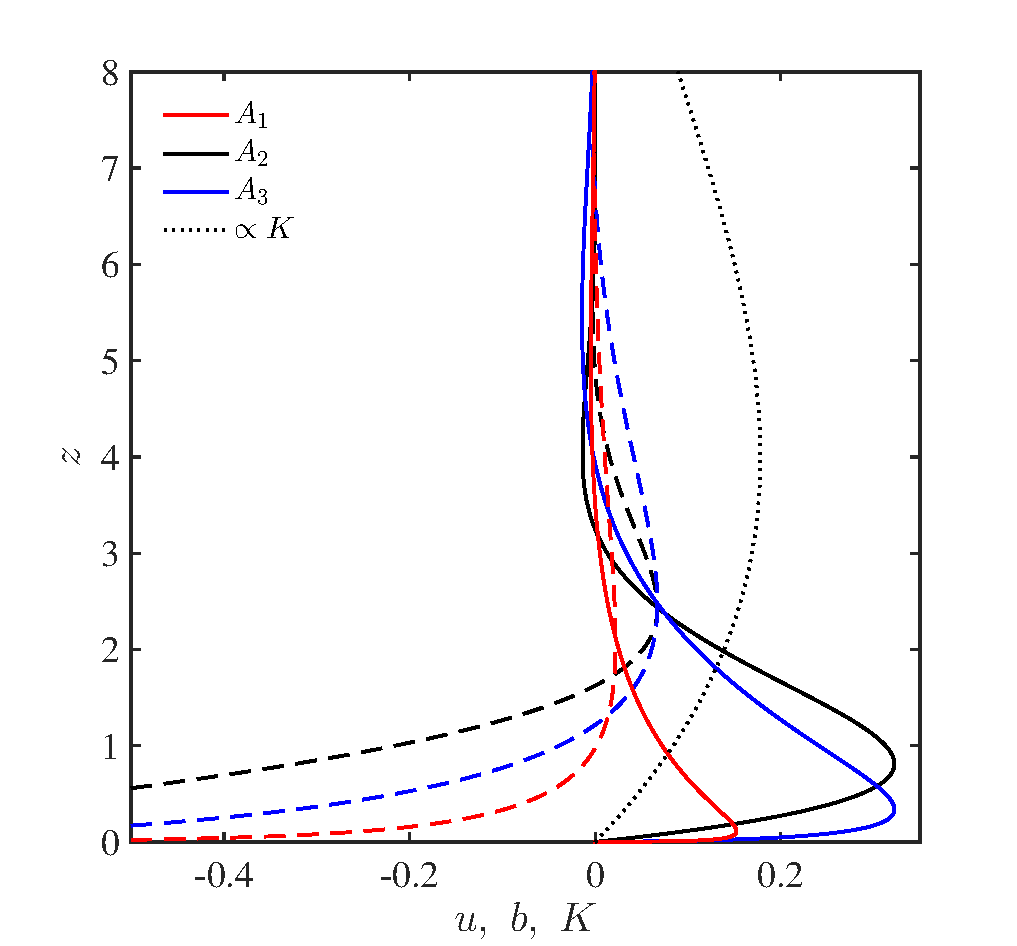
\includegraphics[width= 70.0mm]{comparison_analytic_solutions.eps}
      \caption{Comparison of the proposed analytic solution (A1) against the constant-$K$ (A2) and the WKB solution (A3). $u$ is positive in the down-slope direction. The dashed black line identifies the adopted eddy viscosity $K_M$. The constant-$K$ value is fixed to $K_M^{\mathrm{A2}} = \max(K_M^{\mathrm{A1}})/3$. Velocity profiles $(u)$ are denoted with solid lines whereas buoyancy profiles $(b)$ are denoted by dashed lines. Here $z_0 = 0.001, \, Pr=1$ and $H = 12$. Assuming $\hat{N}=10^{-2} \ \mathrm{(Hz)}$, $\hat{\alpha}=5^{\circ}$ and $\hat{b}_s = -0.1 \ \mathrm{(m \, s^{-2})}$, the corresponding dimensional system, based on $u_* \equiv \hat{u}_* U^{-1}$ from the A1 solution, is characterized by $\hat{z}_0 = 0.08 \ \mathrm{(m)}$ and $\hat{u}_* = 0.18 \ \mathrm{(m \, s^{-1})}$, within the range of commonly observed atmospheric values. 
      A1 is indistinguishable to a corresponding second-order centered finite-difference numerical solution (also exact in double precision arithmetics), therefore the comparison is omitted.}
      \label{fig1}
   \end{center}
\end{figure}
%
In Fig. \ref{fig1} we compare the proposed analytic solution (A1) against the constant-$K$ (A2) and the WKB solution (A3), considering $Pr=1$ (i.e., $\hat{K}_M = \hat{K}_H$).
The constant-$K$ solution is evaluated based on Eqs. \ref{Prandtl_sol}, and the WKB solution is evaluated based on Eqs. \ref{WKB_sol}. 
For the sake of comparison, A1 and A3 are evaluated for the same $z_0$ and $H$ (hence same $K(z)$) parameters, whereas A2 is computed imposing $K_{A2} = \max{(K)}/3$.
$\hat{h}$ is evaluated iteratively in order to match $z_r$ of the A1 solution. Given that the resulting A1 solution is relatively insensitive to the exact $\hat{h}$ (in the neighborhood of the $\hat{h}=\hat{z}_r$ value) only a few iterations are necessary to provide a good approximation of the desired $\hat{K}$.
The chosen $K(z)$ satisfies the constraints defined in \citet{Grisogono2002} for the validity of the WKB method.
A1 shows a remarkably strong inversion in the near surface regions, when compared against its analytical counterparts, suggesting an over-diffusive behavior of both A2 and A3. 
For instance, normalised surface buoyancy gradients of simulation A1 are over an order of magnitude larger than those of A3 ($b_z^{\mathrm{A1}}/b_z^{\mathrm{A3}} = \mathcal{O}(10)$ for $z \rightarrow z_0$).
Nevertheless, $u_z^{\mathrm{A1}} \approx u_z^{\mathrm{A3}}$ for $z \rightarrow z_0$, confirming the better dissipative properties of A3, when compared against the constant-$K$ approach. 
To underline the importance of a decreasing magnitude of eddy diffusivities as the surface is approached, it is worth noting that $u_z^{\mathrm{A1}}/ u_z^{\mathrm{A2}} = \mathcal{O}(10)$. Overall, the proposed normalised solution differs significantly when compared against A2 and A3, in both amplitude and location of extrema. 
Both the height of the LLJ and the peak velocity are significantly reduced, features that are of great importance for an accurate representation of the stable boundary layer and from a parameterisation perspective \citep{Mahrt1998}.
Besides, A1 predicts significantly reduced mass and buoyancy (slope-parallel) fluxes, viz. $\int_0^{H}{u}{\, \mathrm{d}z}$ and $\int_0^{H}{b}{ \, \mathrm{d}z}$, with respect to A2 and A3.


% Z0 DEPENDENCY 
%%%%%%%%%%%%%%%%%%%%%%%%%%%%%%%%%%%%%%%%%%%%%%%%%%%%%%%%%%%%%%%%%

\begin{figure}
    \begin{center}
    \begin{tabular}{c c}
    	\includegraphics[width= 48.0mm]{z0_sensitivity_plot.eps} &
	\includegraphics[width= 48.0mm]{z0_sensitivity_plot_grisogono.eps}
    \end{tabular}
    \caption{Sensitivity of the normalised A1 (left) and A3 (right) solutions to the $z_0$ parameter. Solid lines denote down-slope velocity $(u)$ whereas dashed lines denote buoyancy $(b)$. Fixed parameters: $H=12$, $Pr=1$.}
    %Assuming $N=10^{-2} \ \mathrm{(Hz)}$, $\alpha=30 \ \mathrm{(deg)}$ and $b_s = -0.1 \ \mathrm{(ms^{-2})}$, the resulting dimensional profiles are characterised by $z_{0,1} = 0.0008 \ \mathrm{(m)}, u_{*,1} = 0.09 \ \mathrm{(ms^{-1})}$, $z_{0,2} = 0.01 \ \mathrm{(m)}, u_{*,2} = 0.18 \ \mathrm{(ms^{-1})}$ and $z_{0,3} = 0.3 \ \mathrm{(m)}, u_{*,3} = 0.39 \ \mathrm{(ms^{-1})}$ respectively. A lower portion of the domain is shown for both normalised and dimensional profiles.%
    \label{fig3}
    \end{center}
\end{figure}
%
%\begin{figure}
%    \begin{center}
%    \begin{tabular}{c c}
%    	\includegraphics[width= 48.0mm]{./z0_sensitivity_plot_normalised_grisogono} &
%	\includegraphics[width= 48.0mm]{./z0_sensitivity_plot_grisogono}
%    \end{tabular}
%    \caption{Sensitivity of the normalised A3 solution $(\overline{u},\overline{b})$ to the $\overline{z}_0$ parameter (left) and a corresponding family of dimensional profiles $(u,b)$ (right). Solid lines denote velocity profiles whereas dashed lines denote buoyancy profiles. Choice of model parameters: $\overline{\zeta}^{(i)}=10$, $\overline{z}_{0,1} = 0.0001$, $\overline{z}_{0,2} = 0.001$ and $\overline{z}_{0,3} = 0.01$. To re-dimensionalize the solution we assumed $N=10^{-2} \ \mathrm{(Hz)}$, $\alpha=30 \ \mathrm{(deg)}$ and $b_s = -0.1 \ \mathrm{(ms^{-2})}$. The resulting dimensional profiles are characterised by $z_{0,1} = 0.0002 \ \mathrm{(m)}, u_{*,1} = 0.024 \ \mathrm{(ms^{-1})}$, $z_{0,2} = 0.007 \ \mathrm{(m)}, u_{*,2} = 0.089 \ \mathrm{(ms^{-1})}$ and $z_{0,3} = 0.23 \ \mathrm{(m)}, u_{*,3} = 0.29 \ \mathrm{(ms^{-1})}$ respectively. A lower portion of the domain is shown for both normalised and dimensional profiles.}
%    \label{fig4}
%    \end{center}
%\end{figure}
%
The sensitivity of the solution to variations in the $z_0$ parameter is displayed in Fig. \ref{fig3}.
Since $(u_*,b_*) \propto z_0$, where $b_* \equiv \kappa z b_z$, larger hydrodynamic roughness lengths $(z_0)$ correspond to stronger transfer rates of momentum and buoyancy in the vertical direction, yielding a larger $z_j$ and $\max{(u)}$. 
To highlight differences with respect to the WKB solution, the same $z_0$ sensitivity test is displayed for the A3 solution in Fig. \ref{fig3}.
Because $K \approx z$ in the neighborhood of $z=z_0$, A3 predicts $z_j \approx \pi^2/32+z_0$ and $\max{(u)} = 0.32$.  
A3 is therefore able to describe the $z_0$ (alias $K$) dependency of $z_j$, but predicts a $K$-invariant $\max{(u)}$, as is clear from Fig. \ref{fig3}.
A2 is also characterized by a $K$-invariant $\max{(u)}$.
The proposed solution therefore provides additional insight on the physics of the system, valid within the underlying Monin-Obukhov framework and idealized boundary conditions, suggesting a somewhat different coupling between the velocity and buoyancy fields, when compared to that predicted by previous analytic solutions of the linear Prandtl model. It shows that a larger $z_0$ parameter results in a higher and stronger LLJ ($[z_j,\max{(u)}] \propto z_0$).
Further, since $\hat{L} = \kappa \hat{u}_*/(\hat{N} \sin{\alpha})$, the characteristic scale of the flow $(\hat{L})$ will vary proportionally to $z_0$ for a prescribed $\hat{U},\hat{B},\alpha$ set. 

%Further, given that A1 predics a larger $u_*$, when compared against A2 and A3, the re-dimensionalized solution is characterised by a larger characteristic scale L, as apparent if one compares the dimensional profiles in Fig. \ref{fig3} and \ref{fig4}.  

%Of practical interest from a parameterisation perspective is the relation between the internal and given external parameters of the problem $(u_*,b_*$ and $b_s,N,\alpha,z_0$ respectively).
%From the normalised solution it is possible to compute:
%%
%\begin{eqnarray}
%	\overline{u}_* = \kappa \overline{z}_0 \frac{d \overline{u}}{d\overline{z}}\bigg|_{\overline{z}_0} = f_1(\overline{z}_0) , \hspace{0.5cm}
%	\overline{b}_* = \kappa \overline{z}_0 \frac{d \overline{b}}{d\overline{z}}\bigg|_{\overline{z}_0} = f_2(\overline{z}_0),
%	\label{internal_external_parameters}
%\end{eqnarray}
%%
%where $f_1,f_2$ are universal function of the dimensionless model parameters.
%$f_1$ and $f_2$ are depicted in Figure \ref{fig7}.
%$\overline{z}_0$ is chosen to encompass a vast range of realistic values of the dimensional hydrodynamic roughness length.
%Given the computational burden of evaluating hypergeometric functions, we here provide a valid approximation of $f_1,f_2$, in the form of a power-law, expanded around the solution at $\overline{z}_0=10^{-5}$:
%%
%\begin{eqnarray}
%	\overline{u}_* & = & 0.055 + 0.28 (\overline{z}_0-10^{-5})^{0.46}, \nonumber \\ 
%	\overline{b}_* & = & 0.035 + 0.29 (\overline{z}_0-10^{-5})^{0.33}.
%	\label{f1-f2}
%\end{eqnarray}
%%
%Eqs. \ref{f1-f2}, together with the specified $b_s$ and $N$, allow to compute $u_* = \overline{u}_* \cdot b_s/N$ and $b_* = \overline{b}_*\cdot b_s$.
%
%\begin{figure}
%   \begin{center}
%      \includegraphics[width= 70.0mm]{./u-b_star_z0}
%      \caption{Dependence of the non-dimensional internal parameters $\overline{u}_*, \overline{b}_*$ on $\overline{z}_0$. We here defined $\overline{u}_* = \kappa \overline{z}_0 (d \overline{u}/d\overline{z})|_{\overline{z}_0}$ and $\overline{b}_* = \kappa \overline{z}_0 (d \overline{b} / d\overline{z})|_{\overline{z}_0}$. Results are obtained for $\overline{\zeta}=10$.}
%      \label{fig5}
%   \end{center}
%\end{figure}
%

%For completeness, we also provide simple formula for the computation of $\overline{z}_j$, $\overline{z}_r$, and $\max{(\overline{u})}$, which are of interest for dispersion studies in complex terrains:
%%
%\begin{eqnarray}
%	\overline{z}_j & = & 0.051 + 1.48 (\overline{z}_0-10^{-5})^{0.48}, \nonumber \\ 
%	\overline{z}_r & = & 4.552 + 2.34 (\overline{z}_0-10^{-5})^{0.36}, \\
%	\max{(\overline{u})} & = & 0.107 + 0.23 (\overline{z}_0-10^{-5})^{0.22}. \nonumber
%	\label{f3-f5}
%\end{eqnarray}
%
%Eqs. \ref{f3-f5} are displayed in Fig. \ref{fig6}.
%
%\begin{figure}
%   \begin{center}
%      \includegraphics[width= 70.0mm]{./zj-zr_z0}
%      \caption{Dependence of $\overline{z}_j$, $\overline{z}_r$, and $\max{(\overline{u})}$ on $\overline{z}_0$. Results are obtained for $\overline{\zeta}=10$.}
%      \label{fig6}
%   \end{center}
%\end{figure} 
%



\begin{figure}
    \begin{center}
    \begin{tabular}{c c}
    	\includegraphics[width= 48.0mm]{Pr_sensitivity_plot.eps} &
	\includegraphics[width= 48.0mm]{Pr_sensitivity_plot_grisogono.eps}
    \end{tabular}
    \caption{Sensitivity of the normalised A1 (left) and A3 (right) solutions to the $Pr$ parameter. Solid lines denote down-slope velocity $(u)$ and dashed lines denote buoyancy $(b)$. Displayed solutions correspond to: $H=12$, $z_0 = 0.001$.}
    \label{fig4}
    \end{center}
\end{figure}
%
Under stably stratified environments, pressure fluctuations induced by breaking gravity waves sum to those induced by turbulence, and yield an increase in the total momentum flux, without directly influencing the buoyancy flux \citep{Mahrt1998}. 
This results in turbulent Prandtl numbers that are usually greater than unity. Variations by a factor of 2 for $Pr$, perhaps even more under conditions of strong stratification, are common and that can lead to considerable changes in the shapes of vertical profiles of velocity and buoyancy. 
The sensitivity of the solution to variations in the $Pr$ parameter is displayed in Fig. \ref{fig4}. As before in Fig. \ref{fig3}, the closed form solution (A1) is compared to the WKB solution (A3).
Variations in $Pr$ change the solution throughout the domain for both A1 and A3, larger $Pr$ results in weaker thermal and dynamic boundary-layers, and in a proportional decrease in $u_j$ and $z_j$. 
Such a behavior could have been anticipated, since a larger $Pr$ in conjunction with the constant (imposed) surface buoyancy is expected to result in a lower surface buoyancy flux, i.e. in a lower rate of potential energy injected into the system.

To study the sensitivity of the solution on the $h$ parameter we considered a $\pm 10 \%$ $h$-variation, and results are displayed in Fig. \ref{fig5}.
Despite the non-negligible changes in $K(z)$ in the outer regions of the flow we observe a modest $\approx \pm 0.5 \%$ variation in $\max{(u)}$ and a $\approx \pm 5 \%$ variation in $z_j$, $\min{(u)}$ and $z_r$ (the location of $\min{(u)}$), which is well within the degree of accuracy of the current study. Recall that variations in $h$ lead to the same first order Taylor expansion of $K(z)$ around $z_0$, therefore the inner regions of the flow are relatively insensitive to the exact $h$ value.




% PRACTICAL NOTES 
%%%%%%%%%%%%%%%%%%%%%%%%%%%%%%%%%%%%%%%%%%%%%%%%%%%%%%%%%%%%%%%%%

\section{On the computation of the solution}

%
\begin{figure}
    \begin{center}
    \begin{tabular}{c c}
	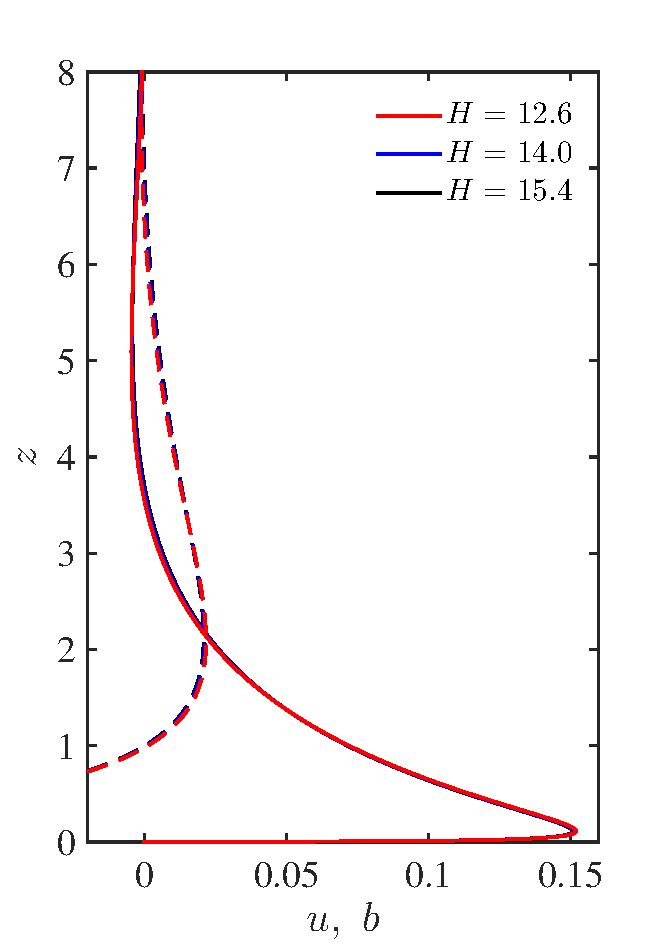
\includegraphics[width= 48.0mm]{H_sensitivity_plot.eps} &
	\includegraphics[width= 48.0mm]{halfwidth_convergence_zj_um.eps}
   \end{tabular}
    \caption{Left plot: Sensitivity of velocity $u$ (solid lines) and buoyancy $b$ (dashed lines) profiles on the $H$ parameter for the A1 solution. Right plot: convergence test, relative percentage error for $z_j$ (red lines) and $\max{(u)}$ (blue lines) as a function of $N$, where $N$ represents the number of terms considered in the truncated $_2F_1$ series. Parameters for the $H$-sensitivity study (left plot): $H_1=11.2$, $H_2=14$, $H_3=16.8$ and $z_0=0.001$.  Parameters for the convergence test (right plot): $z_0 = 0.00001$ (squares), $z_0 = 0.0001$ (circles), $z_0 = 0.001$ (crosses) and $H=14$. We define $e_{z_j} = 100(z^N_j-z_j)/z_j$ and $e_{\max{(u)}} = 100[\max{(u^N)}-\max{(u)}]/\max{(u)}$, where $(\cdot)^N$ represents a quantity computed truncating the $_2F_1$ series to $N$ terms, and where $z_j$ and $\max{(u)}$ represent quantities that are exact in double precision arithmetic. }
    \label{fig5}
    \end{center}
\end{figure}
%
The computation of the Gauss hypergeometric function $_2F_1$ with all its parameters complex is known to be a non-trivial task. Although the $_2F_1$ function is merely a power series expansion (whose implementation is immediate), its use is prone to cancellation and round-off error, which become especially significant for certain ranges of the parameters and of the independent variable \citep{temme2007}.
In our case, the solution $f = b+iu$ is evaluated in $y \in (z_0 / H, 1)$, which is within the radius of convergence $(R)$ of the hypergeometric functions that define $f$ (the radius of convergence of $_2F_1(a,b,c,y)$ is $|y|=1$). 
The solution computed here represents the $_2F_1$ functions as truncated power series, i.e. $_2F_1(a,b,c,y) = [(a)_k(b)_k]/[(c)_k k!] y^k$, where $a,b,c$ are the three input parameters, $(\cdot)_k$ is the Pochhammer symbol and $k!$ denotes the factorial of $k=1,2,\dots N$. 
All computations are performed in double precision arithmetic.
In Fig. \ref{fig5} we display the convergence of the solution, in terms of $z_j$ and $\max{(u)}$, for a given set of $z_0$ values and $H =10$. 
The solution shows sub-logarithmic convergence for both $e_{z_j} = 100(z^N_j-z_j)/z_j$ and $e_{\max{(u)}} = 100[\max{(u^N)}-\max{(u)}]/\max{(u)}$, and clearly, the smaller the $z_0$ parameter, the slower the resulting convergence rate. 
This behavior is justified by the fact that as $z_0$ is reduced, the solution is evaluated closer to $R$, where the convergence of $_2F_1$ in its power series form is known to be retarded.
Despite the slow convergence of the series summation, the evaluation of the solution is stable throughout the range of realistic $z_0$.
Note that the efficacy of the series summation could be much improved by various techniques (e.g., Shanks method, Pad\'e summation, etc.), but such an analysis is beyond the goal of the current study.




%\begin{table}
%\caption{Set of parameters for re-normalisation of the reference solution. The reference normalised solution is computed adopting $H^+ = 10, A^+ = 6.75 \times 10^{-4}, \epsilon^+ =1.5 \times 10^{-3}$.}
%\label{table}
%\centering
%\begin{tabular}{l l l l l l l l}
%\hline
% Value & Ref. & $\alpha1$ & $\alpha_2$ & $N_1$ & $N_2$ & $b_{s,1}$ & $b_{s,2}$ \\
%\hline
%   $\alpha \ (\mathrm{deg})$ & 30 & 15 & 60 & 30 & 30 & 30 & 30  \\
%   $N \ (\mathrm{Hz})$ & 0.01 & 0.01 & 0.01 & 0.005 & 0.02 & 0.01 & 0.01 \\
%   $b_s \ (\mathrm{ms^{-2}})$ & 0.30 & 0.30 & 0.30 & 0.30 & 0.30 & 0.15 & 0.60 \\
%\hline
%\end{tabular}
%\end{table}

%To get acquainted with the proposed normalisation Fig. \ref{fig2} proposes a set of re-dimensionalized velocity profiles $u \ \mathrm{(ms^{-1})}$ from a reference normalised solution.
%We propose a reference dimensional solution, characterised by $\alpha = 30 \ \mathrm{(deg)}, N = 0.01 \ \mathrm{(Hz)}$ and $b_s = -0.1  \ \mathrm{(ms^{-2})}$, and consider variations in both sloping angle $\alpha$, imposed buoyancy frequency $N$ and imposed surface buoyancy $b_s$ (see Table \ref{table}).
%Variations in the sloping angle $\alpha$ result in a modification of the normalisation constant $L \propto \sin^{-1/2}$ which acts as a stretching of the independent variable $z$ (no effects on $\max{(u)}$). 
%In particular, the steeper the angle, the smaller the characteristic scales of the flow will become.
%Variations in the background stratification, viz. $N$, will modify both $L \propto N^{-1/2}$ and $U \propto N^{-1}$, yielding changes in the system, whose lengths and velocities will tend to decrease (increase) with increasing (decreasing) $N$.
%Further, variations in the prescribed surface buoyancy $b_s$ will scale both buoyancy and velocity profiles accordingly, since $b(z) \propto b_s$ and $u(z) \propto b_s$.


% ####################################################################
\section{Conclusions}
%
A closed form solution of the Prandtl model equations has been proposed herein, valid for O'Brien-type eddy diffusivities and constant Prandtl number. 
The solution is for katabatic flows and is an adaptation of the solution proposed in \citet{Nieuwstadt1983a} for the Ekman-layer equations, generalized to account for constant $Pr \neq 1$.
Its characteristics have been discussed assuming transfer coefficients for momentum and buoyancy in accordance to Monin-Obukhov similarity (albeit the solution lend itself to more general $K$-parameterisations). 
The dependence of the normalised solution on the model dimensionless parameters $Pr$ and $\hat{z}_0 \hat{N}^2 \hat{b}_s^{-1}$ has been tested and compared against corresponding WKB solutions. 
For the same geometrical and physical parameters, profiles show significant variations in both phase and amplitude of extrema with respect to their WKB counterparts: stronger surface gradients (inversely proportional to $Pr$) are combined with overall reduced slope-parallel fluxes, and the LLJ is further displaced toward the wall.
In addition, its peak velocity, LLJ height, and surface gradients proved to be highly sensitive to variations of the dimensionless parameter $\hat{z}_0 \hat{N}^2 \hat{b}_s^{-1}$, highlighting a more complex coupling between the velocity and buoyancy fields.
Despite the slow convergence of the series summation, which can however be accelerated through various techniques, the evaluation of the solution is stable throughout the range of realistic $z_0$.
The proposed model can be of use to validate numerical or patched / matched solutions of the Prandtl equations, and to improve future stable boundary layer parameterisations, when coupled with other parts of the boundary layer physics.


% ####################################################################
\section{Acknowledgements}
%
This research was funded by the Swiss National Science Foundation (SNSF-200021-134892), the Competence Center for Environmental Sustainability (CCES-SwissEx) of the ETH domain, and the NSERC Discovery Grant program. 
We are grateful to the peer reviewers whose comments helped to improve the overall quality of the manuscript.

%\appendix?


% BibTeX users please use one of
\bibliographystyle{spbasic_nourl}      % basic style, author-year citations
%\bibliographystyle{spmpsci}      % mathematics and physical sciences
%\bibliographystyle{spphys}       % APS-like style for physics
\bibliography{/Users/mg/Phd/papers/bib_files/library}






\end{document}

